% !TEX program = xelatex

\documentclass[10pt,a4paper,fontset=fandol]{ctexart}

\usepackage[left=1.20cm,right=1.20cm,top=1.00cm,bottom=1.00cm]{geometry}
\usepackage{fontawesome}
\usepackage{graphicx}
\usepackage{tabularx}
\usepackage{array}
\usepackage{enumitem}
\usepackage{titlesec}
\usepackage{xcolor}
\usepackage[hidelinks]{hyperref}
\usepackage{setspace}

\setmainfont[
  Path = fonts/Main/ ,
  Extension = .otf ,
  UprightFont = *-regular ,
  BoldFont = *-bold ,
  ItalicFont = *-italic ,
  BoldItalicFont = *-bolditalic ,
  SmallCapsFont = Fontin-SmallCaps
]{texgyretermes}

\pagestyle{empty}
\setlength{\parindent}{0pt}
\setlength{\parskip}{0pt}
\setstretch{1.0}
\hypersetup{colorlinks=false}

\definecolor{accent}{HTML}{1F4E79}
\definecolor{bodygray}{HTML}{222222}

\titleformat{\section}
  {\large\bfseries\color{accent}}
  {}{0pt}{}
  [\vspace{0.12em}\titlerule]
\titlespacing*{\section}{0pt}{0.55em}{0.32em}

\setlist[itemize]{
  leftmargin=1.25em,
  itemsep=0.05em,
  topsep=0.06em,
  parsep=0pt,
  partopsep=0pt
}

\newcommand{\entry}[3]{
  \textbf{#1}\hfill #2\\
  #3
}

\newcommand{\paper}[4]{
  \textbf{#1}\hfill #2\\
  #3\\
  {\small #4}
  \vspace{0.08em}
}

\newcommand{\project}[4]{
  \textbf{#1}\hfill #2\\
  {\small #3}
  \begin{itemize}
    #4
  \end{itemize}
}

\newcommand{\award}[2]{#1\hfill #2\\}

\begin{document}
\color{bodygray}

\begin{tabularx}{\textwidth}{@{}m{2.45cm}@{\hspace{0.65cm}}>{\raggedright\arraybackslash}X@{\hspace{0.45cm}}>{\raggedright\arraybackslash}X@{}}
  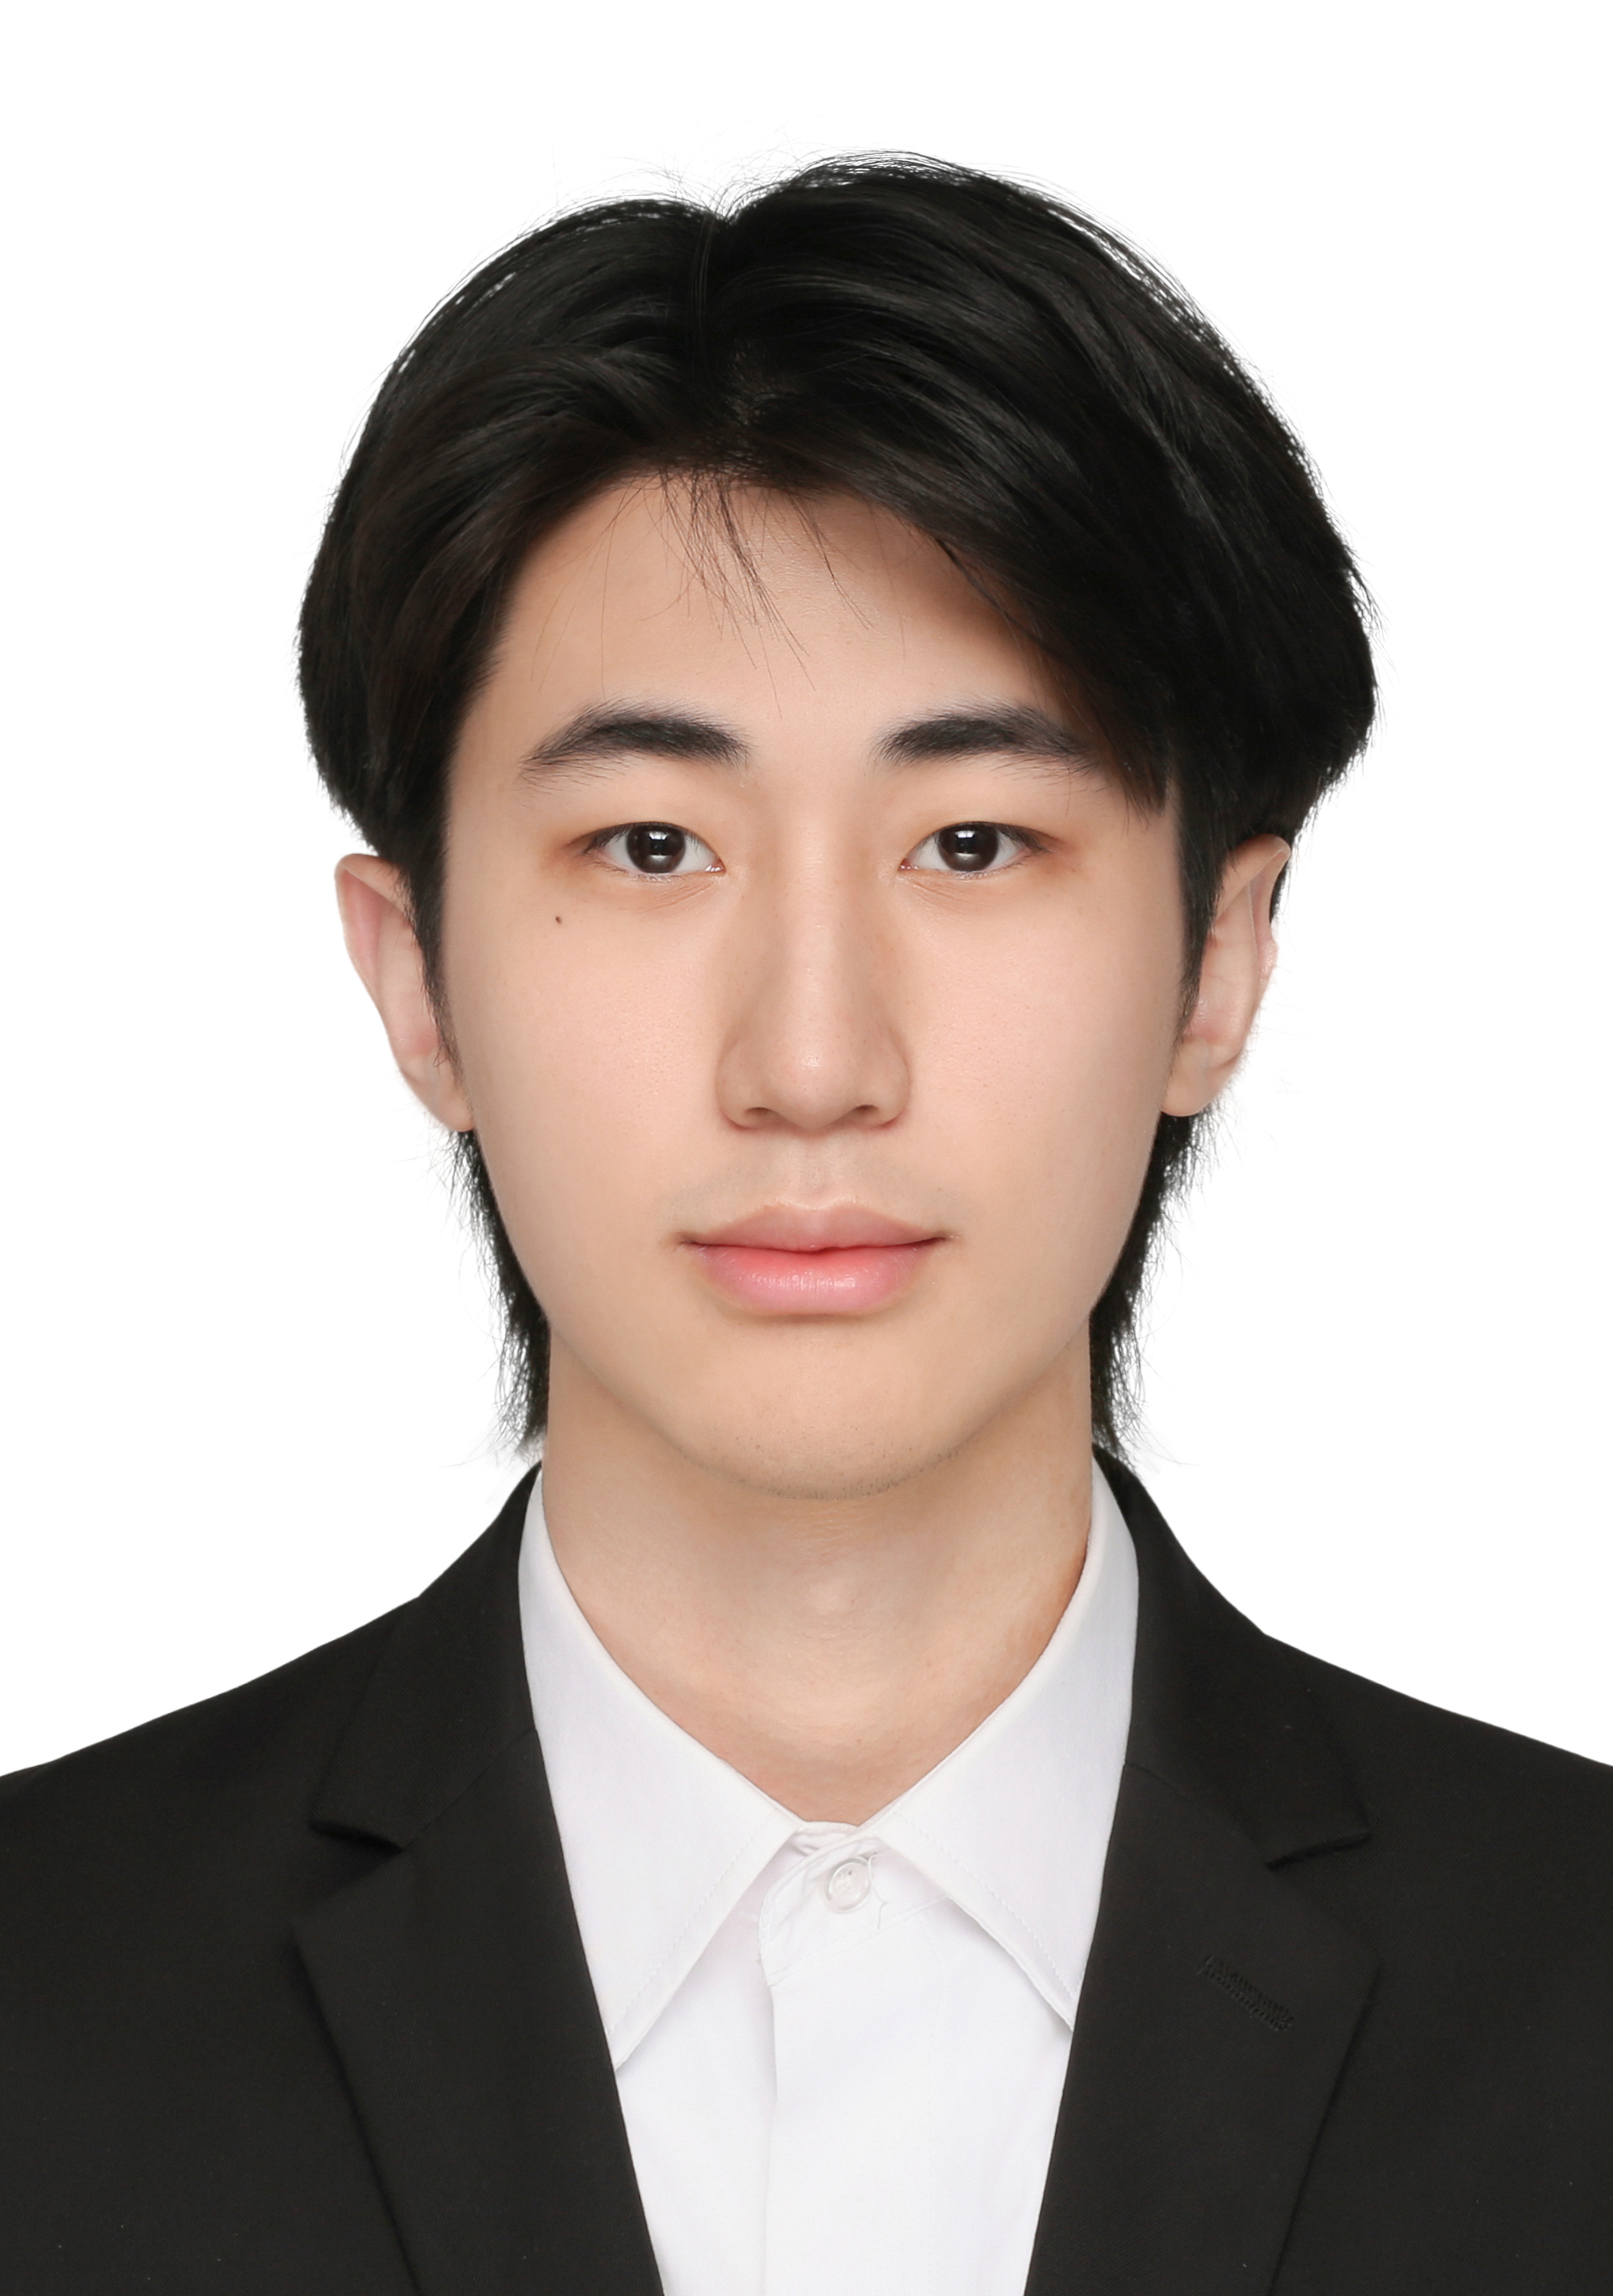
\includegraphics[width=2.35cm,height=3.10cm,keepaspectratio]{changyue.jpg}
  &
  \begin{tabular}[c]{@{}l@{}}
    {\Huge\bfseries 常越}\\[0.35em]
    香港科技大学（广州）博士生\\
    研究方向：多模态大模型、具身智能、机器人
  \end{tabular}
  &
  \begin{tabular}[c]{@{}l@{}}
    \faEnvelope\ \href{mailto:ychang500@connect.hkust-gz.edu.cn}{ychang500@connect.hkust-gz.edu.cn}\\
    \faPhone\ +86 18977312314\\
    \faGithub\ \href{https://github.com/CYandYue}{CYandYue}\\
    \faLink\ \href{https://cyandyue.github.io/HomePage/}{个人主页}
  \end{tabular}
\end{tabularx}

\vspace{0.18em}

\section{\texorpdfstring{{\normalfont\faGraduationCap}\ 教育背景}{教育背景}}
\entry{香港科技大学（广州），博士，人工智能/计算机方向}{2025.03 -- 至今}
{导师：谢思宏教授；研究方向为 LLM/MLLM 与 Robotics，聚焦长程导航、三维场景图与多模态决策。}

\vspace{0.12em}
\entry{哈尔滨工业大学（深圳），本科，自动化专业}{2021.09 -- 2025.07}
{主修课程：线性代数、自动控制原理、数字图像处理、机器视觉、数/模电等；GPA 3.533/4.0。}

\section{\texorpdfstring{{\normalfont\faFileTextO}\ 论文与研究成果}{论文与研究成果}}
\paper{RAG-3DSG: Enhancing 3D Scene Graphs with Re-Shot Guided Retrieval-Augmented Generation}{ECCV 2026}
{\textbf{Yue Chang}, Rufeng Chen, Zhaofan Zhang, Yi Chen, Yifan Tian, Sihong Xie}
{提出面向 3D Scene Graph 的检索增强生成框架，通过 re-shot guided retrieval 补充场景图缺失信息，提升开放世界三维场景理解与机器人任务执行中的语义表达质量。}

\paper{PSG-Nav: Probabilistic Scene Graph Navigation via Multiverse Decision Making}{ICML 2026}
{Rufeng Chen*, \textbf{Yue Chang}*, Xiaqiang Tang, Hechang Chen, Sihong Xie}
{共同一作；围绕概率场景图导航，将不确定场景建模与多分支决策结合，用于复杂环境下的机器人长程规划。}

\paper{A Unified Hallucination Mitigation Framework for Large Vision-Language Models}{TMLR}
{\textbf{Yue Chang}*, Liqiang Jing*, Xiaopeng Zhang*, Zhang Yue}
{一作工作；构建 LVLM 幻觉检测与缓解框架，负责主要 idea 生成、代码实现、实验设计与论文写作，代码开源于 \href{https://github.com/CYandYue/Dentist}{Dentist}。}

\paper{Just-In-Time Scene Graph Growth: Combating Perceptual Saturation in Long-Horizon Robotics}{arXiv 2026}
{\textbf{Yue Chang}, Rufeng Chen, Yifan Tian, Dazhi Huang, Zhaofan Zhang, Yi Chen, Wenze Zhang, Li Chen, Hui Xiong, Sihong Xie}
{针对长程机器人任务中的感知饱和问题，探索按需增长的场景图更新机制，服务持续环境理解与任务规划。}

\paper{LH-AVLN: A Benchmark for Long-Horizon Audio-Visual-Language Navigation}{arXiv 2026}
{Rufeng Chen, \textbf{Yue Chang}, Zili Shao, Zhaofan Zhang, Hechang Chen, Hui Xiong, Sihong Xie}
{参与构建长程音频-视觉-语言导航基准，覆盖多模态感知、语言指令理解与长程决策评测。}

\section{\texorpdfstring{{\normalfont\faBriefcase}\ 科研与实习经历}{科研与实习经历}}
\project{香港科技大学（广州）具身智能/多模态研究}{2025.03 -- 至今}
{博士生，导师：谢思宏教授}
{
  \item 围绕 LLM/MLLM 与机器人结合开展研究，重点关注 3D Scene Graph、长程导航、多模态决策与开放世界语义理解。
  \item 产出多篇论文，包括 ECCV 2026、ICML 2026 录用论文及 2026 年 arXiv 预印本，承担问题定义、方法设计、实验实现与论文写作工作。
}

\project{University of Texas at Dallas 实验室}{2023.09 -- 2024.10}
{Research Intern}
{
  \item 研究 Large Vision-Language Models 的幻觉检测与缓解问题，系统调研 LVLM 幻觉来源、评测协议与缓解策略。
  \item 作为第一作者完成统一幻觉缓解框架，负责核心方法设计、代码实现、实验分析与论文写作，论文被 TMLR 接收。
}

\project{深圳若愚科技有限公司}{2023.07 -- 2023.10}
{算法工程师实习生}
{
  \item 使用 CLIP 进行数据预处理与数据增强，参与实际业务场景中的多模态数据构建与模型适配。
  \item 部署并微调多模态大模型，完成 YOLO-v8 在华为开发板上的部署与推理验证。
}

\section{\texorpdfstring{{\normalfont\faTrophy}\ 竞赛获奖}{竞赛获奖}}
\award{RoboMaster 超级对抗赛步兵组，全国一等奖}{2023}
\award{RoboMaster 超级对抗赛团体赛，全国二等奖}{2023}
\award{“矿蛟杯”物流科技创意赛，全国二等奖}{2023}
\award{中国机器人及人工智能大赛，全国二等奖}{2023}
\award{RoboMaster 超级对抗赛哨兵组，全国三等奖}{2023}
\award{BOTEC 国际智能机器人技术挑战赛，全国三等奖}{2022}
\award{RoboMaster 超级对抗赛区域赛/高校联盟赛，省级一等奖}{2023}
\award{本科三等奖学金}{2022}

\end{document}
